\documentclass[12pt,a4paper]{article}

\usepackage[backend=bibtex,style=alphabetic]{biblatex}
\addbibresource{references.bib}
\usepackage{makecell}
\renewcommand\theadfont{\bfseries}
\usepackage{tabularx}
\usepackage{array}
\usepackage{amssymb}
\newcolumntype{Y}{>{\centering\arraybackslash}X}
\usepackage{float}
\usepackage{graphicx}
\usepackage{listings}
\usepackage[utf8]{inputenc}
\usepackage[english]{babel}
\usepackage[T1]{fontenc}
\usepackage{geometry}
\usepackage{setspace}
\usepackage{lmodern}
\usepackage{tocloft}
\usepackage{titlesec}
\usepackage[hidelinks]{hyperref}
\geometry{a4paper, margin=2.5cm}
\onehalfspacing
\lstset{
    basicstyle=\ttfamily\small,
    breaklines=true,
    columns=fullflexible,
    showstringspaces=false
}

\titleformat{\section}{\Large\bfseries}{\thesection}{1em}{}
\titleformat{\subsection}{\large\bfseries}{\thesubsection}{1em}{}
\titleformat{\subsubsection}{\normalsize\bfseries}{\thesubsubsection}{1em}{}

\begin{document}

\begin{titlepage}
\centering

\vspace*{1cm}

{\Large \textbf{BABEȘ-BOLYAI UNIVERSITY OF CLUJ-NAPOCA}}\\[0.2cm]
{\large FACULTY OF MATHEMATICS AND COMPUTER SCIENCE}\\[0.2cm]
{\large SPECIALIZATION: COMPUTER SCIENCE}\\
{\large (IN GERMAN)}\\

\vspace{4cm}

{\LARGE \textbf{BACHELOR THESIS}}\\[1.5cm]
{\Large ALPRo: An AI-Assisted ALPR Platform for Romanian Traffic Services}

\vfill

\begin{flushleft}
Supervisor\\
Associate Prof. PhD Sanda-Maria AVRAM
\end{flushleft}

\begin{flushright}
\textit{Author:}\\
Jitariu Rareș-Ștefan
\end{flushright}

\vspace{1cm}
\centering
2026

\end{titlepage}

\begin{titlepage}
\centering

\vspace*{1cm}

{\Large \textbf{BABEȘ-BOLYAI-UNIVERSITÄT CLUJ-NAPOCA}}\\[0.2cm]
{\large FAKULTÄT FÜR MATHEMATIK UND INFORMATIK}\\[0.2cm]
{\large SPEZIALISIERUNG AUF INFORMATIK}\\
{\large (IN DEUTSCHER SPRACHE)}\\

\vspace{4cm}

{\LARGE \textbf{LIZENZARBEIT}}\\[1.5cm]
{\Large ALPRo: Eine KI-unterstützte ALPR-Plattform für rumänische Verkehrsdienste}

\vfill

\begin{flushleft}
Wissenschaftlicher Leiter\\
Dozentin PhD Sanda-Maria AVRAM
\end{flushleft}

\begin{flushright}
\textit{Absolvent:}\\
Jitariu Rareș-Ștefan
\end{flushright}

\vspace{1cm}
\centering
2026

\end{titlepage}

\begin{titlepage}
\centering

\vspace*{1cm}

{\Large \textbf{UNIVERSITATEA BABEȘ-BOLYAI CLUJ-NAPOCA}}\\[0.2cm]
{\large FACULTATEA DE MATEMATICĂ ȘI INFORMATICĂ}\\[0.2cm]
{\large SPECIALIZAREA INFORMATICĂ}\\
{\large (ÎN LIMBA GERMANĂ)}\\

\vspace{4cm}

{\LARGE \textbf{LUCRARE DE LICENȚĂ}}\\[1.5cm]
{\Large ALPRo: O platformă ALPR asistată de inteligență artificială pentru serviciile de trafic din România}

\vfill

\begin{flushleft}
Coordonator\\
Conf. Univ. Dr. AVRAM Sanda-Maria
\end{flushleft}

\begin{flushright}
\textit{Absolvent:}\\
Jitariu Rareș-Ștefan
\end{flushright}

\vspace{1cm}
\centering
2026

\end{titlepage}



\newpage
\thispagestyle{empty}
\mbox{}

\newpage
\begin{center}
\rule{\textwidth}{0.4pt}
\vspace{0.3cm}

\textbf{\large ABSTRACT}

\vspace{0.3cm}
\rule{\textwidth}{0.4pt}
\end{center}

\vspace{0.8cm}
\onehalfspacing

Automatic License Plate Recognition (ALPR) systems are increasingly used in traffic administration, parking verification, law enforcement support, and vehicle-related administrative workflows. Many existing solutions are commercial, difficult to adapt, or not designed around local registration rules. This thesis presents \textbf{ALPRo}, a full-stack, AI-assisted ALPR platform built for Romanian license plate formats and for the practical needs of police, parking, and insurance users.

The application is organized as a modular system composed of a React frontend, a Spring Boot backend, a PostgreSQL database, and a separate FastAPI-based machine learning service. The recognition workflow supports both image uploads and video processing. Detected plate strings are normalized and validated against Romanian registration rules, including standard, diplomatic, temporary, military, MAI, probe, local, and unknown plate categories. The platform also includes a review queue where detections can be confirmed or rejected before they become part of the operational history.

Artificial intelligence is used in ALPRo as a controlled support layer rather than as a replacement for deterministic validation. The OpenAI API is integrated in two main areas. First, a role-aware Copilot allows users to ask natural language questions about vehicles, parking sessions, insurance policies, detections, and audit events, then guides them directly to the relevant part of the application. Second, an AI-assisted vehicle recognition component suggests visible attributes such as make, model, color, and body type from representative vehicle images. These features make the interface faster to use while keeping the plate validation logic explicit and auditable.

The platform also provides JWT authentication, role-based access control, audit logging, parking session management by city zone, insurance policy management, vehicle case reports, PDF export, and CSV audit export. Docker Compose is used to run the frontend, backend, database, and machine learning service together, which simplifies development and demonstration.

The work focuses on building and evaluating a practical prototype. The evaluation covers photo recognition, video recognition, Romanian plate validation, AI-assisted vehicle attribute recognition, and Copilot query handling. The result is a localized ALPR ecosystem that combines computer vision, rule-based validation, and AI-assisted interaction for Romanian traffic service workflows.
\newpage
\tableofcontents
\newpage

\section{Introduction}

The growth of urban traffic has increased the amount of vehicle-related information that public and private operators need to process every day. Parking operators must verify whether a vehicle has an active parking session in the correct zone. Police users need fast access to vehicle records and detection history. Insurance users need structured access to vehicle and policy information. In all these cases, the license plate is often the simplest connection between a physical vehicle and the digital records associated with it.

Automatic License Plate Recognition (ALPR) systems address this problem by detecting and reading license plates from images or video streams. They are already used in tolling, access control, parking enforcement, traffic monitoring, and smart city systems. Still, many available solutions are closed, expensive, or designed as generic products that are not easy to adapt to local formats and workflows. Romania introduces its own constraints: county prefixes, Bucharest-specific formats, temporary plates, diplomatic plates, MAI and military formats, and locally issued plates that do not always follow the standard pattern.

This thesis presents \textbf{ALPRo}, a web-based ALPR platform developed around these Romanian requirements. The project does not treat recognition as an isolated computer vision problem. Instead, it connects recognition with the operational modules that would normally use the result: vehicle lookup, parking verification, insurance policy management, detection review, audit history, and reporting. This makes the application useful not only for detecting a plate, but also for deciding what should happen after the plate has been detected.

The system follows a modular architecture. The frontend is implemented in React and provides role-specific screens for police, parking, and insurance users. The backend is implemented with Spring Boot and manages authentication, authorization, business rules, persistence, audit logging, and communication with the machine learning service. PostgreSQL stores the operational data, while a FastAPI service handles image and video recognition tasks. Docker Compose is used to run the services together during development and demonstration.

A central part of ALPRo is the validation of Romanian plate formats. After a plate candidate is detected, the text is normalized and checked against explicit rules for standard, diplomatic, temporary, probe, military, MAI, local, and unknown plates. This rule-based layer is important because it prevents the system from accepting arbitrary OCR text as a valid Romanian registration number. It also makes the behavior easier to explain and review.

The project also includes AI-assisted features based on the OpenAI API. A Copilot component allows users to ask natural language questions and receive direct guidance inside the application. For example, a user can ask for vehicles without insurance, active parking sessions, or the history of a specific plate, and the assistant can translate the request into application-level actions or links. A second AI component analyzes selected vehicle images and suggests visible attributes such as make, model, color, and body type. These features are designed to reduce manual searching and make the interface easier to use, without removing the deterministic validation rules from the recognition pipeline.

The goal of this thesis is therefore to design, implement, and evaluate a practical ALPR ecosystem for Romanian traffic service scenarios. The evaluation focuses on the behavior of the photo and video recognition workflows, the correctness of Romanian plate validation, the usefulness of the review process, and the role of AI-assisted interaction inside the application.

The following chapters present the theoretical background of ALPR and related systems, the requirements and architecture of ALPRo, the implementation of its main modules, the testing and evaluation process, and the conclusions drawn from the prototype.

\section{Theoretical Background}

\subsection{Automatic License Plate Recognition in Intelligent Transportation Systems}

Automatic License Plate Recognition (ALPR), also referred to as Automatic Number Plate Recognition (ANPR), is a computer vision task that extracts vehicle registration information from images or video streams. The technology is used in traffic monitoring, tolling, access control, parking management, public safety, and other intelligent transportation scenarios. Classical ALPR systems are usually described as a pipeline composed of image acquisition, plate localization, character segmentation, character recognition, and post-processing \cite{Du2013,Mufti2021}. Although the terminology differs slightly across studies, the core idea remains the same: visual data must first be reduced to a plate region, then converted into a structured textual identifier.

The practical difficulty of ALPR comes from the uncontrolled nature of road environments. A license plate can appear at different distances, under different lighting conditions, at oblique angles, partially occluded, dirty, blurred by movement, or compressed by low-quality video. Surveys of ANPR systems show that older image processing methods, such as edge detection, thresholding, morphology, and template matching, can work in constrained settings but tend to degrade when the environment changes \cite{Mufti2021}. This is one reason why modern systems increasingly use machine learning and deep learning models for localization and recognition.

In the context of smart cities, ANPR is not only a recognition problem, but also a data infrastructure problem. Tang et al. describe ANPR as a sensing technology that supports urban applications such as traffic analysis, enforcement, transport planning, and operational decision-making \cite{Tang2022}. This broader perspective is important for ALPRo because the detected plate is not the final goal of the application. The plate acts as an entry point into workflows such as vehicle lookup, parking verification, insurance checking, audit history, and detection review.

\subsection{Deep Learning and YOLO-Based Plate Detection}

Deep learning changed ALPR by replacing many handcrafted detection steps with trainable object detection models. The YOLO family of detectors is particularly relevant because it is designed for real-time object detection and can localize objects in a single forward pass. Laroca et al. demonstrated that YOLO-based systems can perform ALPR in real time and can be trained for multiple stages of the recognition pipeline, including vehicle detection, plate detection, and character recognition \cite{Laroca2018}. Later work by the same group introduced a layout-independent approach that combines plate detection with layout classification and post-processing rules, showing that recognition can be improved when visual models are combined with structural knowledge about plate formats \cite{Laroca2021}.

This combination of learned detection and rule-based interpretation is especially relevant for localized systems. A generic object detector can identify candidate plate regions, but the system still needs to decide whether the recognized text is a valid plate for the target country. Recent YOLO-based research continues to emphasize the trade-off between speed, accuracy, and robustness. Al-Hasan et al. use YOLOv8 in an ANPR system designed for Qatar and discuss the balance between accuracy and computational efficiency \cite{AlHasan2024}. Ultralytics documentation also presents YOLOv8 as a family of models intended for object detection, segmentation, classification, pose estimation, and related tasks, with several model sizes that allow different speed-accuracy trade-offs \cite{UltralyticsYOLOv8}.

Research focused on difficult ALPR conditions shows that robustness remains a central challenge. Sultan et al. discuss ALPR under challenging conditions, where illumination, viewing angle, blur, and environmental variation affect detection and recognition \cite{Sultan2023}. Similarly, Meesad and Thumthong emphasize the need for regionally adaptive ALPR systems and show that even strong deep learning models must be adjusted to local plate characteristics, fonts, scripts, and environmental conditions \cite{Meesad2025}. These observations support the design choice in ALPRo to combine automated recognition with explicit Romanian validation rules and a review step for uncertain results.

\subsection{Romanian License Plate Formats and Rule-Based Validation}

Romanian license plates follow a structure that is regular enough to be validated, but varied enough to require more than a single simple pattern. Standard plates usually contain a county code or the Bucharest code, followed by two or three digits and three letters. However, Romanian traffic also includes diplomatic plates, temporary plates, probe plates, military plates, Ministry of Internal Affairs plates, electric vehicle plates with green characters, and locally issued plates. The legal basis for the composition and use of different plate categories is found in national road traffic regulations, including Government Decision no. 1391/2006 and the more recent MAI Order no. 181/2024 regarding registration, deregistration, provisional circulation authorization, and plates for testing or provisional use \cite{HG1391,Ordin181}.

For an ALPR application, these rules are not only descriptive; they are part of the recognition process. If a model returns a string that resembles a plate visually but violates the Romanian format, the system should not treat it as a valid registration number. Rule-based validation therefore acts as a safety layer after recognition. In ALPRo, detected text is normalized and then classified into categories such as standard, diplomatic, temporary, probe, military, MAI, local, or unknown. This classification makes the result easier to understand for users and prevents random OCR output from entering operational workflows as if it were a verified plate.

Romanian-specific ALPR research also confirms the value of local adaptation. Buleu, Robu, and Filip present a deep learning system for Romanian ALPR using YOLOv12 and PaddleOCR, with a dataset collected from vehicles registered in Romania and functionality for county identification \cite{Buleu2025}. Their work supports the idea that local plate syntax, vehicle context, and regional data matter when building a reliable recognition pipeline. ALPRo follows the same general principle, even though its application focus is broader: recognition is connected to review, parking, insurance, vehicle records, audit logs, and AI-assisted navigation.

\subsection{Video Processing and Vehicle Attribute Recognition}

Video-based ALPR introduces different constraints from single-image recognition. A video can contain many frames of the same vehicle, so processing every frame with the same level of detail can be inefficient. At the same time, video gives the system more opportunities to obtain a clearer view of the plate. Ribeiro and Hirata propose an efficient video-based ALPR approach that uses YOLO and visual rhythm to select a representative frame instead of relying on redundant processing of many frames \cite{Ribeiro2025}. This idea is relevant for ALPRo's video workflow, where the application should be responsive enough for demonstration and practical use without consuming unnecessary compute resources.

Resource constraints are also important in real deployments. Padmasiri et al. study ALPR for resource-constrained environments and show that deployment on edge or low-power hardware requires attention to model size, latency, and processing limitations \cite{Padmasiri2022}. Although ALPRo is packaged as a Docker-based prototype rather than a dedicated edge device, the same concern appears in the video workflow: the system should avoid unnecessary calls and should aggregate repeated detections instead of treating every frame as an independent event.

A related but distinct task is vehicle attribute recognition. Knowing the plate number is often enough for lookup, but make, model, color, and body type can help users interpret a detection, especially when checking whether a detected vehicle matches existing records. Parsa et al. discuss video-based vehicle surveillance using vision-language models for license plate, make, and model recognition in uncontrolled video settings \cite{Parsa2025}. Their work shows that modern vision-language systems can assist with semantic vehicle attributes, although they also remain sensitive to image quality and viewpoint. In ALPRo, AI-assisted attribute recognition is therefore treated as a supportive suggestion rather than as a final authority.

\subsection{Smart Parking, Access Control, and Operational Workflows}

Parking is one of the most natural application areas for ALPR. In urban areas, a plate can link a vehicle to a parking session, a zone, a payment, or a possible violation. Smart parking research connects vehicle identification with IoT, machine learning, occupancy detection, and real-time user interfaces. Alymani et al. describe smart parking systems as part of smart city infrastructure, emphasizing benefits such as reducing time spent searching for parking, improving traffic flow, and supporting more efficient use of urban space \cite{Alymani2025}. This supports the design of ALPRo's parking module, where sessions are not only stored as isolated entries but are associated with zones and can be searched by plate.

The same principle applies to police and insurance workflows. A police user may need to inspect a vehicle case, previous detections, parking status, or insurance information. An insurance user may need to verify whether a vehicle has an active policy. These scenarios require controlled access to data, because the same plate can connect to information with different sensitivity levels. For this reason, ALPRo uses role-based access and audit logging as part of the system design. The ALPR result is therefore integrated into a larger operational model, not displayed as a standalone computer vision output.

\subsection{Natural Language Interfaces and AI-Assisted Querying}

A growing direction in software systems is the use of large language models as natural language interfaces over structured data. Instead of asking users to navigate several screens manually, an assistant can help interpret a request and map it to a controlled action. This approach is especially useful when the application contains several related modules, such as vehicles, detections, parking sessions, insurance policies, and audit events.

Recent research on LLM-based database interaction explores how natural language can be transformed into database operations or tool calls. AskDB presents an LLM agent for interacting with relational databases through natural language and emphasizes schema-aware prompting and multi-step task decomposition \cite{Phan2025AskDB}. FinAI Data Assistant proposes a more constrained approach: instead of generating arbitrary SQL, the assistant routes user requests to a small set of vetted parameterized queries, improving reliability, latency, and cost control \cite{Kim2025FinAI}. This second idea is particularly close to ALPRo's design philosophy. The assistant should not freely invent database queries; it should map user intent to safe application-level operations.

The OpenAI Responses API supports text and image inputs and allows models to use tools or custom functions, while OpenAI's function calling documentation describes how models can produce structured arguments for external functions rather than executing application logic themselves \cite{OpenAIResponses2026,OpenAIFunctionCalling2026}. In ALPRo, this distinction is important. The Copilot does not replace backend authorization or business rules. It helps the user formulate a request, chooses an appropriate supported action, and returns a useful answer or navigation target. The backend remains responsible for authentication, authorization, validation, and data retrieval.

This theoretical foundation positions ALPRo as a hybrid application. The recognition pipeline uses computer vision and validation rules to identify Romanian plates. The operational modules use role-based data access to connect the detected plate to real workflows. The AI components support interaction and visible vehicle attribute recognition, but the system keeps deterministic validation and backend security rules at the center of the design.

\section{System Requirements and Design}

\subsection{Functional Requirements}

The functional requirements of ALPRo were defined around the operations that a traffic service application must support after a license plate has been detected. The system is not limited to reading a plate from an image; it connects the recognition result to vehicle records, parking sessions, insurance policies, review decisions, reports, and audit events.

\begin{itemize}
  \item \textbf{Authentication and role-based access:} The system must allow users to log in with secure credentials and must assign each user a role. The active role determines which pages, actions, and backend endpoints are available.

  \item \textbf{Photo-based plate detection:} Police users must be able to upload a vehicle image and receive one or more detected Romanian plate candidates. The result must include the normalized plate number, plate type, and editable vehicle information such as brand, model, owner, color, and body type.

  \item \textbf{Video-based plate detection:} Police users must be able to upload a video and start a processing job. The system must aggregate repeated detections across frames, store the most relevant results, and expose the job status and final detections through the frontend.

  \item \textbf{Romanian plate validation and classification:} The application must normalize and validate detected text according to Romanian plate rules. The system must classify supported categories such as standard, diplomatic, temporary, probe, military, MAI, local, or unknown.

  \item \textbf{Human review of detections:} Automatic detections must be available in a review queue. Police users must be able to confirm or reject photo and video detections, optionally adding a reason. This requirement prevents uncertain automatic output from becoming operational data without human control.

  \item \textbf{Vehicle case lookup:} Police users must be able to search a plate and view a consolidated vehicle case. The case should include vehicle data, insurance information, parking history, detection history, and relevant audit events.

  \item \textbf{Parking session management:} Parking operators must be able to register vehicle entry and exit events, including the parking zone. Police users may consult already registered parking sessions by plate, but they must not create or modify parking records.

  \item \textbf{Insurance policy management:} Insurance users must be able to create and update insurance policies associated with a plate. Police users may consult insurance status when investigating a vehicle case, but policy management remains restricted to the insurance role.

  \item \textbf{Audit history:} The system must record relevant operational actions, such as police lookups and insurance changes. Police users must be able to filter and export audit events for later inspection.

  \item \textbf{AI-assisted vehicle attributes:} When an image contains enough visual information, the system should use an AI-assisted component to suggest vehicle attributes such as make, model, color, and body type. These suggestions must remain editable by the user.

  \item \textbf{Copilot interaction:} The application must provide a role-aware assistant that can interpret natural language requests and guide users toward the correct module or result. The assistant should use controlled application actions instead of bypassing backend rules.

  \item \textbf{Reporting and exports:} Police users must be able to generate a vehicle report in PDF format, while audit data should be exportable in CSV format for administrative review.
\end{itemize}

These requirements define ALPRo as an operational prototype rather than a simple OCR demonstration. Each recognition result is connected to a controlled workflow, and each workflow is limited by role and purpose.

\subsection{Non-Functional Requirements}

The non-functional requirements describe the expected qualities of the platform. They are important because ALPR systems process sensitive vehicle-related data and must remain understandable, maintainable, and reliable during demonstrations and testing.

\begin{itemize}
  \item \textbf{Usability:} The interface must be clear for non-technical users. Police, parking, and insurance users should see only the modules that are relevant to their work, reducing confusion and preventing accidental misuse.

  \item \textbf{Responsiveness:} Photo detection should return a result quickly enough for interactive use. Video detection can take longer, but it must expose job status and final results so that the user does not have to guess whether processing is still running.

  \item \textbf{Cost-aware AI usage:} OpenAI-based features should be used only where they add value. The Copilot should focus on short, structured requests, while vehicle attribute recognition should run only on representative images rather than on every video frame.

  \item \textbf{Data integrity:} The system must normalize plate numbers consistently and must not accept arbitrary OCR text as a valid Romanian plate. The review queue adds another integrity layer by allowing uncertain detections to be checked manually.

  \item \textbf{Security and role isolation:} Backend endpoints must enforce authorization based on the authenticated user's role. Frontend hiding is useful for usability, but backend restrictions remain the real security boundary.

  \item \textbf{Auditability:} Important actions must be stored with user, action type, timestamp, and relevant details. This makes later inspection possible and discourages uncontrolled access to sensitive records.

  \item \textbf{Maintainability:} The application should keep clear boundaries between frontend components, backend controllers, service classes, repositories, and external integrations. This separation makes future changes easier to implement and test.

  \item \textbf{Portability:} The main services should run together through Docker Compose. This makes the project easier to demonstrate, rebuild, and move between development machines.

  \item \textbf{Extensibility:} The system should allow new plate categories, AI actions, reports, or external integrations to be added without rewriting the entire application.
\end{itemize}

\subsection{User Roles and Use Cases}

ALPRo uses three main operational roles: \texttt{POLICE}, \texttt{PARKING}, and \texttt{INSURANCE}. The application interface and backend access rules are built around these roles.

\begin{itemize}
  \item \textbf{Police user:} This role has access to photo and video detection, detection review, vehicle case lookup, read-only parking search, insurance consultation, audit history, dashboard statistics, and PDF reports. The police user is the main role for investigation and validation workflows.

  \item \textbf{Parking operator:} This role manages parking sessions. The operator can register entries and exits, choose the parking zone, and search existing sessions. The role does not have access to detection review, vehicle case reports, insurance management, or audit pages.

  \item \textbf{Insurance user:} This role manages insurance policies and searches policy status by plate. The insurance user can create and update policy records, but cannot operate parking sessions or review detections.
\end{itemize}

Each role corresponds to a different operational use case. The police role needs a broad view over the vehicle case, while parking and insurance roles are intentionally narrower. This separation keeps the application closer to a real institutional workflow, where access is based on responsibility rather than convenience.

\begin{figure}[H]
    \centering
    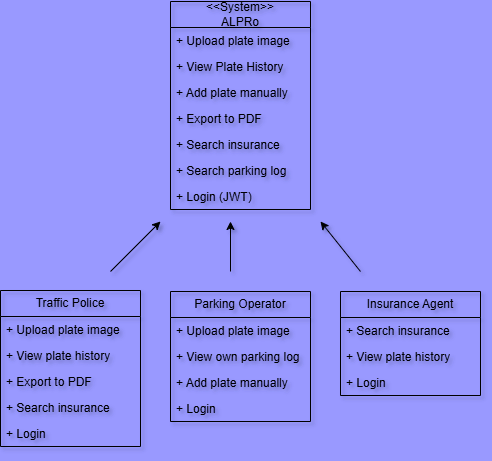
\includegraphics[width=0.9\textwidth]{images/diagrama3-1.png}
    \caption{Use case diagram for ALPRo, showing the operational roles and their main responsibilities.}
    \label{fig:use-case}
\end{figure}

\subsection{Security and Access Control}

Security is a central design concern because the application stores vehicle records, insurance information, parking sessions, detection history, and audit events. ALPRo uses a combination of authentication, authorization, validation, and audit logging.

\textbf{Authentication} is implemented with JSON Web Tokens (JWT). After login, the backend issues a token that contains the user's identity and role. The frontend sends this token with subsequent API requests, and the backend validates it before processing protected operations.

\textbf{Role-based access control} is enforced on backend routes. For example, only police users can access detection review and video processing. Parking operators can create parking entries and exits, while police users can only consult parking sessions. Insurance users can create and update policies, while police users can consult policy status but cannot manage policy records.

\textbf{Frontend route protection} improves the user experience by hiding pages that do not belong to the active role. This is not treated as the main security layer, because a user could still attempt to call an endpoint manually. The backend authorization rules remain responsible for enforcing the real access boundary.

\textbf{Validation} is applied to plate text and user input. Plate normalization and Romanian validation rules reduce the risk of storing invalid recognition results. For operational forms such as parking and insurance, required fields are checked before data is saved.

\textbf{Audit logging} records important actions such as vehicle lookups and insurance changes. These logs support later review and make sensitive operations easier to inspect. In the prototype, audit logging is especially useful for demonstrating how the application separates ordinary data access from actions that should leave a record.

Together, these mechanisms make ALPRo suitable as an academic prototype that handles realistic data flows while keeping access control and review decisions explicit.

\newpage



\section{Implementation Architecture}

The implementation of ALPRo follows a modular architecture in which each component has a clearly defined responsibility. The application is not implemented as a single monolithic OCR script, but as a web platform that combines a Spring Boot backend, a React frontend, a PostgreSQL database and a separate FastAPI service for machine learning inference. This separation is important because the ALPR pipeline contains tasks with different technical requirements: user authentication and business rules are handled by the backend, interactive screens are handled by the frontend, persistent operational data is stored in the database, while computationally expensive image and video analysis is isolated in the ML service.

The complete application can be started through Docker Compose. This makes the deployment reproducible and allows the backend, frontend, database and ML service to run in the same environment without requiring manual configuration of each component. From the perspective of the user, ALPRo behaves as a single application. From the perspective of the implementation, however, each request passes through several layers: the browser sends authenticated requests to the backend, the backend checks the user role and business rules, the ML service is called only when image or video inference is required, and the result is persisted in PostgreSQL before being returned to the interface.

The following subsections describe the main implementation layers and the way in which they collaborate.

\subsection{Overall System Structure}

The architecture contains four main services:

\begin{itemize}
    \item the React frontend, responsible for the user interface, navigation, form validation and role-specific screens;
    \item the Spring Boot backend, responsible for authentication, authorization, business logic, persistence, audit logs and integration with external AI services;
    \item the PostgreSQL database, responsible for storing users, plates, detections, video jobs, parking sessions, insurance policies and audit events;
    \item the FastAPI ML service, responsible for detecting and reading license plates from images and videos.
\end{itemize}

The backend is the central coordination layer. The frontend does not communicate directly with the database or with the ML service. This design prevents the browser from bypassing business rules and keeps sensitive functionality behind backend authorization checks. For example, a police user can consult parking sessions that already exist in the database, but cannot create parking entries. This restriction is enforced in the backend, not only in the interface.

The ML service is separated from the backend because computer vision dependencies are different from the dependencies required by Spring Boot. The service loads the plate detector and OCR components, exposes HTTP endpoints for inference and returns structured JSON responses. The backend then validates the plate text using Romanian registration rules and decides whether the detection can be accepted directly or should be sent to manual review.

OpenAI integration is also placed in the backend. ALPRo uses it for two distinct purposes: the Copilot assistant, which interprets natural language requests and maps them to safe application actions, and vehicle attribute recognition, where a representative vehicle image is sent to the model in order to estimate make, model, color and body type. OpenAI is not used as the primary plate detector. This keeps the cost controlled and preserves the deterministic Romanian validation logic.

\subsection{Backend Layer}

The backend is implemented in Java using Spring Boot. It contains controllers, services, repositories, DTOs, domain models and security components. The controller layer exposes REST endpoints, while the service layer contains the actual application logic. This separation keeps request handling independent from business decisions and makes the code easier to extend.

The main backend controllers include \texttt{OcrController}, \texttt{VideoJobController}, \texttt{DetectionReviewController}, \texttt{LicensePlateController}, \texttt{PoliceLookupController}, \texttt{ParkingHistoryController}, \texttt{InsuranceController}, \texttt{AuditController}, \texttt{DashboardController} and \texttt{CopilotController}. Each controller is responsible for one module of the application. For instance, \texttt{OcrController} handles photo detections, \texttt{VideoJobController} handles video processing requests, \texttt{DetectionReviewController} handles manual confirmation or rejection of uncertain detections, while \texttt{PoliceLookupController} builds the vehicle case view used by police users.

The service layer contains classes such as \texttt{OcrService}, \texttt{VideoJobService}, \texttt{VideoJobProcessorService}, \texttt{RomanianPlateValidator}, \texttt{ParkingService}, \texttt{PoliceLookupService}, \texttt{DashboardService}, \texttt{AuditLogService} and \texttt{CopilotService}. This layer coordinates the main workflows of the platform. A photo recognition request, for example, is not only a call to an OCR endpoint. The backend receives the image, calls the ML service, validates the candidate plate, stores the detection, optionally enriches the result with vehicle attributes and returns a response that can be shown in the interface.

This separation is important because the machine learning result is treated as a candidate, not as the final application decision. The backend adds the operational rules that the ML service does not know by itself: Romanian plate validation, review status, user permissions, persistence, audit logging and optional AI-based vehicle attributes. In this way, the recognition pipeline remains connected to the rest of the system instead of being an isolated image-processing script.

The communication between the Spring Boot backend and the ML service is implemented as a multipart HTTP request. This keeps the detector outside the main backend and allows the computer vision component to be replaced or improved without changing the operational modules of the application. Listing~\ref{lst:ml-client-image} shows the image inference call used by the backend client.

\begin{lstlisting}[language=Java, caption={Backend call to the ALPR machine learning service}, label={lst:ml-client-image}]
public MlAlprResult detectPlate(File imageFile) throws IOException {
    RequestBody multipartBody = new MultipartBody.Builder()
        .setType(MultipartBody.FORM)
        .addFormDataPart("image", imageFile.getName(),
            RequestBody.create(imageFile,
                MediaType.parse("application/octet-stream")))
        .build();

    Request request = new Request.Builder()
        .url(inferEndpoint())
        .post(multipartBody)
        .build();

    try (Response response = httpClient.newCall(request).execute()) {
        if (!response.isSuccessful()) {
            throw new IOException("ALPR ML service error: "
                + response.code());
        }
        JSONObject json = new JSONObject(response.body().string());
        return new MlAlprResult(
            json.optString("plateText", null),
            readOptionalDouble(json, "confidence"),
            readBbox(json.optJSONObject("bbox")),
            readCandidates(json.optJSONArray("candidates")));
    }
}
\end{lstlisting}

\subsection{Machine Learning Service}

The ML service is implemented with FastAPI and exposes dedicated endpoints for image and video inference. The service loads a YOLO-based license plate detector and applies OCR on the cropped plate regions. For image recognition, the pipeline receives an uploaded image, detects candidate plate regions, crops the best candidates, applies OCR and returns the most likely plate text together with internal metadata.

For video recognition, the service processes the video frame by frame according to configurable sampling parameters. Processing every frame would be expensive and unnecessary for most traffic videos, so the service uses a frame step and a maximum processed frame count. Detected plates are tracked across nearby frames using bounding-box overlap and text stability. This reduces duplicate detections and avoids calling OCR on every single frame when the same vehicle remains visible for several frames.

The video pipeline also returns a representative vehicle image when available. This image is useful for vehicle attribute recognition, because the OpenAI model receives a larger visual context than the plate crop itself. The system therefore avoids asking the AI model to infer the car model from the license plate region only, which would be unreliable. Instead, it sends a cropped vehicle context selected from the video track or from the uploaded photo.

The ML response includes information such as the detected plate text, confidence values, bounding boxes and optional vehicle images. Not all of this information is shown to end users. For example, numerical confidence values and bounding boxes are kept mainly as internal technical data. The frontend can display a live rectangle around a detected plate during video playback because it helps the operator understand where the detection happened, but the final user-oriented screens and reports focus on the plate, type, vehicle information and operational status.

\subsection{Pipeline Tuning for Image and Video Recognition}

The tuning performed in ALPRo does not modify the internal YOLO architecture. Instead, the system adapts the complete recognition pipeline around the detector. This approach is appropriate for the scope of the application, because the goal is not to design a new object detection model from scratch, but to integrate an existing detector into a Romanian ALPR workflow that is reliable enough for operational use.

For image recognition, tuning is applied after the detector and OCR components produce candidate results. The backend does not automatically accept every text returned by OCR. Candidate plate texts are normalized, checked against Romanian plate formats and rejected when they do not match any supported category. This post-processing step improves the practical quality of the system, because a visually plausible OCR result is not necessarily a valid Romanian registration number.

The photo pipeline also benefits from separating candidate detection from final application decisions. YOLO and OCR are responsible for identifying possible plate regions and reading text, while the backend decides whether the result can be used directly, whether it should be stored with a known plate type, or whether it should remain unavailable for operational use. In this sense, the tuning is not limited to a numerical confidence threshold. It combines ML output with deterministic validation rules.

For video recognition, the main tuning problem is different. Processing every frame would be expensive and would often produce repeated detections of the same vehicle. ALPRo therefore uses configurable parameters such as frame sampling and maximum processed frames. These parameters reduce processing time while still allowing the system to inspect enough frames for visible plates. The video pipeline also groups repeated appearances, so that the same plate is not treated as a completely new result every time it appears in consecutive frames.

This design creates a practical balance between accuracy, speed and cost. Lower sampling intervals may detect more difficult plates, but they increase processing time. Higher sampling intervals are faster, but they may miss plates that appear only briefly or are visible in a small number of frames. The chosen configuration therefore represents an operational compromise rather than a purely theoretical optimum.

The same idea is used for AI-based vehicle attribute recognition. The application does not send every video frame to OpenAI. Instead, it uses selected representative images and limits the number of AI calls per video job. This keeps the feature useful while controlling cost and avoiding unnecessary repeated analysis of the same vehicle.

Overall, the recognition quality in ALPRo is improved through pipeline-level tuning: model output filtering, Romanian plate validation, video sampling, repeated-detection aggregation and controlled AI enrichment. This is different from training a new YOLO model, but it is a relevant engineering optimization for a complete ALPR application.

\subsection{Romanian Plate Validation and Review Flow}

A central part of ALPRo is the Romanian plate validation layer. The ML service can return OCR text, but OCR text alone is not enough. Romanian registration plates have several official and semi-structured formats, including standard county plates, diplomatic plates, temporary plates, PROBE plates, military plates and Ministry of Internal Affairs plates. The backend therefore uses \texttt{RomanianPlateValidator} to normalize and classify candidate plate text before it becomes part of the operational database.

The validation process first removes unnecessary spaces, converts letters to uppercase and then checks the candidate against known formats in a fixed order. The order matters because some formats can be visually similar. ALPRo checks diplomatic plates, MAI plates, military plates, PROBE plates, temporary plates, standard plates and local plates before returning an unknown classification. For standard plates, the county code is also checked against the list of valid Romanian county codes. This prevents accepting a text that matches a generic regular expression but starts with an invalid county prefix.

The application uses the following plate categories: \texttt{STANDARD}, \texttt{DIPLOMATIC}, \texttt{TEMPORARY}, \texttt{PROBE}, \texttt{MILITARY}, \texttt{MAI}, \texttt{LOCAL} and \texttt{UNKNOWN}. These categories are stored through the domain model and can be used later in filters, review screens and reports.

Not every detection is trusted automatically. If the system receives a plate candidate that is invalid, ambiguous or operationally important, the result can be placed in the review queue. The \texttt{DetectionReviewController} allows police users to confirm, reject or reopen detections. This design is useful because ALPR systems operate in imperfect visual conditions. A human operator can correct the final decision without changing the underlying ML service.

\subsection{Frontend Layer}

The frontend is implemented in React and is organized around role-specific modules. The application uses protected routes so that each user type sees only the screens that are relevant to that role. The main routes include the dashboard, detections, vehicle cases, parking, insurance, audit and authentication screens. A floating Copilot widget is available after login and can help the user navigate or search through the system.

The dashboard provides a compact operational overview. Instead of exposing technical details, it presents useful summaries such as detections waiting for review, parking sessions, active policies and recent audit events. The detection module contains three tabs: photo recognition, video recognition and manual review. The vehicle module allows police users to search for a complete vehicle case by plate number. The parking module is used differently depending on the role: parking operators can create and close parking sessions, while police users can only consult existing sessions. The insurance module allows insurance users to manage policies and police users to verify policy status. The audit module is restricted to police users and provides a readable history of important actions.

The frontend also adapts technical results into human-facing language. Detection confidence values are not shown in normal photo results because they are not useful for most operators. Vehicle colors returned by AI are translated into Romanian and displayed with natural capitalization. Bounding boxes are hidden from normal pages and exported reports, except for the real-time video overlay where they help the operator visually confirm the detected plate.

The route protection is handled both in the frontend and in the backend. Frontend protection improves usability by hiding inaccessible screens, while backend annotations such as \texttt{@PreAuthorize} enforce the actual security rules. This double layer prevents accidental access and also makes the interface easier to understand.

\subsection{Database Model}

The PostgreSQL database stores both recognition data and operational data. The model is organized around the license plate number, because this is the common element used by the detection pipeline, the vehicle case page, parking sessions, insurance checks and audit history. This choice makes the plate number the practical link between computer vision results and the operational modules of the application.

Instead of storing detections as isolated OCR outputs, ALPRo connects them with the rest of the vehicle context. Photo detections are stored together with their review status and optional AI vehicle attributes. Video processing is represented through processing jobs and individual detections extracted from those jobs. Parking and insurance records are stored as separate operational modules, but they can be queried by plate number when a police user opens a vehicle case. User accounts and roles are stored separately, while audit events keep a history of relevant searches, confirmations and administrative actions.

This structure supports the main investigative workflow of the application. When a plate is searched, the backend can build a vehicle case by combining identity data, recent photo detections, video appearances, parking sessions, insurance records and audit entries. This is more useful than a simple OCR history table, because it connects recognition results with operational context and allows the user to understand the situation of a vehicle from a single screen.

\subsection{Authentication, Authorization and Audit}

Authentication is based on JSON Web Tokens. After a successful login, the backend returns a token that contains the user identity and role. The frontend stores the token and sends it with authenticated requests. The backend validates the token through the Spring Security configuration and loads the corresponding user details before executing protected endpoints.

ALPRo uses three application roles: \texttt{POLICE}, \texttt{PARKING} and \texttt{INSURANCE}. Police users can perform plate recognition, review detections, search vehicle cases and consult parking and insurance information. Parking users can manage parking sessions. Insurance users can manage insurance policies. This role model reflects the idea that several institutions can use the same ALPR platform, but not all of them should have the same permissions.

Authorization is enforced through backend annotations. For example, photo and video recognition endpoints are restricted to police users, parking creation endpoints are restricted to parking users, and insurance management endpoints are restricted to insurance users. Some endpoints are intentionally shared. Police users can consult parking history and insurance status because these records are relevant during a vehicle check, but they cannot modify parking sessions or insurance policies.

Audit logging is used to record important actions. The system stores events such as vehicle lookups, detection confirmations, detection rejections, insurance checks and other operational actions. The audit page presents these events in readable Romanian labels instead of raw technical action names. This makes the module understandable for users and also supports later analysis of who accessed or changed relevant information.

\subsection{OpenAI-Based Assistance}

ALPRo integrates OpenAI in two places. The first integration is the Copilot assistant. The user can ask natural language questions such as searching a plate, opening the review queue, checking insurance information or navigating to a dashboard module. The backend sends the message and the user role to an OpenAI-powered planning component, receives a structured intent and then executes only the safe actions allowed for that role. The assistant therefore does not directly control the application. It proposes an intent, while \texttt{CopilotService} validates and executes the decision using existing backend services.

This approach is safer than allowing a language model to generate arbitrary database queries. The possible actions are limited to known intents, such as police lookup, parking lookup, insurance lookup, review queue, dashboard navigation or audit lookup. If the requested action is not allowed for the current role, the backend returns a refusal or a help response. This keeps the assistant useful without bypassing the role-based security model.

The second integration is vehicle attribute recognition. After a successful image or video detection, the backend may send a representative vehicle image to OpenAI in order to estimate make, model, body type and color. The result is treated as a suggestion, not as an official truth. The interface presents the suggestion in a user-friendly format and the operator can use it as additional context when building or reviewing a vehicle case.

The model is not retrained for this task. Instead, the application adapts the general vision-language model to the ALPRo context through prompt engineering and a constrained JSON response format. This is important because the application does not need a free-form image description. It needs a conservative operational suggestion that can be stored, displayed and manually corrected. Listing~\ref{lst:vehicle-prompt} shows the prompt used for this purpose.

\begin{lstlisting}[language=Java, caption={Prompt used for vehicle attribute recognition}, label={lst:vehicle-prompt}]
private String buildPrompt() {
    return """
        You assist a Romanian ALPR application. Analyze only
        the visible vehicle, not the license plate text or any
        personal data.

        Return JSON only, with exactly these keys:
        {
          "make": string or null,
          "model": string or null,
          "color": Romanian color name with first letter uppercase,
          "bodyType": string or null,
          "confidence": number between 0 and 1,
          "reasoning": short Romanian explanation
        }

        Rules:
        - Do not infer make or model from the license plate number.
        - If the logo, body shape, or image quality is unclear,
          use null values.
        - Prefer conservative answers over invented vehicle details.
        """;
}
\end{lstlisting}

Both OpenAI integrations are designed with cost control in mind. The application does not call OpenAI for every processed video frame. Instead, vehicle attribute recognition is performed on selected representative images, and Copilot calls happen only when the user sends a message. The deterministic plate validation logic remains inside the backend, which means that the core Romanian plate classification does not depend on a paid language model call.



\newpage



\section{Testing and Evaluation}

The evaluation of ALPRo must cover two dimensions: the technical quality of the recognition pipeline and the correctness of the operational workflows built around that pipeline. Since the current version of the system contains photo recognition, video recognition, Romanian plate validation, manual review, role-based modules, OpenAI-assisted vehicle attributes and a natural language Copilot, the evaluation cannot be reduced to OCR accuracy alone.

This chapter describes the testing strategy used for the prototype and defines the measurements that should be completed before the final version of the thesis is submitted. Numerical results are intentionally not fabricated in this draft. The final values should be filled in only after running the system on a documented test set.

\subsection{Functional Testing}

Functional testing verifies whether the main modules behave according to the requirements defined earlier in the thesis. The tests are organized around user roles and application workflows.

For police users, the tested workflows include photo detection, video job upload, detection review, vehicle case lookup, insurance consultation, parking consultation, audit viewing and PDF export. The expected behavior is that police users can investigate a plate and review detections, but cannot operate parking sessions or manage insurance policies.

For parking users, the tested workflows include opening a parking session, closing a parking session, searching existing sessions and viewing parking-related dashboard information. The expected behavior is that parking operators can manage sessions but cannot access police detection tools or insurance management screens.

For insurance users, the tested workflows include searching policy records, creating policies, updating policies and checking policy status. The expected behavior is that insurance users can manage insurance data but cannot access detection review, video recognition or police audit screens.

The following table summarizes the main functional test groups:

\begin{table}[H]
\centering
\begin{tabular}{|p{4cm}|p{6cm}|p{4cm}|}
\hline
\textbf{Test group} & \textbf{Purpose} & \textbf{Expected result} \\
\hline
Authentication & Validate login and JWT handling & Valid users receive a token; invalid credentials are rejected \\
\hline
Role-based access & Check module visibility and backend permissions & Each role can access only allowed workflows \\
\hline
Photo detection & Upload image and process plate candidates & Valid candidates are stored or sent to review \\
\hline
Video detection & Upload video and process sampled frames & Detections are grouped and exposed in the video results view \\
\hline
Review queue & Confirm or reject uncertain detections & Review status is updated and audited \\
\hline
Vehicle case lookup & Search a plate across modules & The case combines detections, parking, insurance and audit context \\
\hline
Copilot & Ask natural language requests & The assistant returns safe role-aware actions or explanations \\
\hline
\end{tabular}
\caption{Functional test groups for ALPRo}
\end{table}

\subsection{Recognition Evaluation Plan}

The recognition evaluation should be performed on a controlled dataset of Romanian plate images and videos. The dataset should include standard plates, temporary plates, diplomatic plates, PROBE plates, MAI plates, military plates and difficult examples such as blurred, angled, partially occluded or low-light plates. Each sample should have a manually verified ground-truth label.

For photo recognition, the measured metrics are:

\begin{itemize}
    \item plate detection rate: the percentage of images in which a valid plate was returned by the full backend workflow;
    \item exact plate recognition accuracy: the percentage of images where the full normalized plate matched the ground truth;
    \item plate type classification accuracy: the percentage of images assigned to the expected Romanian category;
    \item average client-observed processing time per image.
\end{itemize}

The photo dataset used for the first evaluation contained 20 images of Romanian vehicles under mostly frontal or slightly angled conditions. The complete backend endpoint \texttt{/api/ocr/full} was used, so the measured time includes upload handling, backend orchestration, ML inference and enabled vehicle-attribute enrichment. The system returned a valid plate for 18 images and failed to return a valid plate for 2 images. All 18 returned plates matched the manually labeled ground truth.

\begin{table}[H]
\centering
\begin{tabular}{|p{6cm}|p{4cm}|p{4cm}|}
\hline
\textbf{Metric} & \textbf{Result} & \textbf{Notes} \\
\hline
Total photo samples & 20 & Manually labeled ground truth \\
\hline
Images with valid detected plate & 18/20 & 90.0\% detection rate \\
\hline
Exact plate matches & 18/20 & 90.0\% exact accuracy \\
\hline
Plate type matches & 18/20 & 90.0\% over the full photo set \\
\hline
Average processing time & 2729 ms/image & Client-observed request duration \\
\hline
\end{tabular}
\caption{Photo recognition evaluation results}
\end{table}

For video recognition, the evaluation measures both raw detection quality and operational usefulness. A video can contain the same vehicle across many frames, so evaluating every frame independently is not enough. The first video evaluation pass was executed on 14 short converted MP4 clips using the real backend video job workflow. All 14 jobs completed successfully. Before ground-truth comparison, the system produced detections in 8 videos, returned 15 unique detected plate strings and stored 38 raw detection records. The average processing wait time was 28418 ms per video.

These values describe raw system output. Manual inspection of the clips identified approximately 19 plate appearances that were readable or partially readable by eye. However, the video quality was low: many plates were small in the frame, affected by motion, compression and distance, and some were difficult to read even manually. For this reason, the video experiment is treated as an indicative robustness evaluation rather than a strict accuracy benchmark. The result still shows that the asynchronous video workflow completed reliably and produced useful detections in more than half of the clips.

\begin{table}[H]
\centering
\begin{tabular}{|p{5cm}|p{4cm}|p{5cm}|}
\hline
\textbf{Metric} & \textbf{Result} & \textbf{Notes} \\
\hline
Video jobs completed & 14/14 & All uploaded clips completed successfully \\
\hline
Videos with detected plates & 8/14 & Raw output before ground-truth comparison \\
\hline
Unique detected plate strings & 15 & Across all evaluated videos \\
\hline
Raw video detection records & 38 & Includes repeated appearances across frames or tracks \\
\hline
Average video processing time & 28418 ms/video & Backend job wait time observed by the evaluation script \\
\hline
Strict video recall & Not reported & Ground truth was approximate due to low video readability \\
\hline
\end{tabular}
\caption{Raw video recognition evaluation results}
\end{table}

\subsection{Romanian Plate Validation Tests}

The Romanian validation layer can be tested independently from image recognition. This is useful because it isolates the deterministic part of the system from the ML component. Test cases should include valid and invalid examples for each supported category.

Examples of validation cases include:

\begin{itemize}
    \item standard plates such as \texttt{CJ01ABC}, \texttt{CJ123ABC}, \texttt{B12XYZ} and \texttt{B123XYZ};
    \item diplomatic plates such as \texttt{CD123101}, \texttt{TC156234} and \texttt{CO205113};
    \item temporary plates such as \texttt{CJ012345};
    \item PROBE plates such as \texttt{CJ101PROBE};
    \item military plates such as \texttt{A12345};
    \item MAI plates such as \texttt{MAI123456};
    \item invalid county codes and malformed strings that should be classified as \texttt{UNKNOWN}.
\end{itemize}

This validation test set is important because it demonstrates that the application does not rely only on generic OCR output. It also proves that the system understands Romanian-specific registration formats and rejects plausible but invalid strings.

The current controlled validation test contains 36 cases: 22 valid plate examples, 10 invalid examples and 4 examples where the plate must be extracted from longer OCR-like text. All 36 cases passed, resulting in a 100\% success rate for the deterministic Romanian validation component on this test set. After tightening the local plate rule, the full backend regression suite also passed with 55 tests, 0 failures and 0 errors.

\subsection{AI Feature Evaluation}

The OpenAI-based features should be evaluated separately from the license plate recognition pipeline. The Copilot assistant was tested with 12 controlled operational prompts using the police role. The prompts covered vehicle lookup, parking lookup, insurance lookup, review queue access, dashboard navigation, audit access and general module navigation. The expected result was not free-form creativity, but correct intent classification and useful deep links inside the application.

\begin{table}[H]
\centering
\begin{tabular}{|p{6cm}|p{4cm}|p{4cm}|}
\hline
\textbf{Metric} & \textbf{Result} & \textbf{Notes} \\
\hline
Total Copilot prompts & 12 & Controlled operational prompts \\
\hline
Correct intent classifications & 11/12 & 91.7\% \\
\hline
Correct deep links & 11/12 & 91.7\% \\
\hline
Overall correct responses & 11/12 & 91.7\% \\
\hline
Average response time & 2129 ms/prompt & Client-observed request duration \\
\hline
\end{tabular}
\caption{Copilot evaluation results}
\end{table}

The only failed prompt was an underspecified navigation request, \texttt{vreau vehicule}, where the assistant returned a help response instead of direct navigation. This is acceptable for a prototype because it avoids taking an uncertain action when the request is too vague.

Vehicle attribute recognition should also be treated as an assistant feature. The model may suggest make, model, color and body type, but these results are not official records. In this prototype, these suggestions are used as supporting information in the interface and in the vehicle case workflow, not as authoritative registry data.

Cost behavior was considered in the design. OpenAI is not called for every video frame. It is called only for selected representative images or when the user sends a Copilot message. This keeps API usage proportional to user actions and unique detections rather than to the total number of processed frames.

\subsection{Observed Limitations}

The expected limitations of the prototype are typical for an ALPR system tested in real conditions. Very small plates, motion blur, strong reflections, dirt, occlusion and steep camera angles can reduce recognition quality. Video processing also requires balancing speed and accuracy: a smaller frame step processes more frames and can improve recall, but it increases processing time.

Another limitation is that vehicle attribute recognition depends on the quality of the vehicle crop. If the image contains only the plate or a very small part of the vehicle, make and model recognition becomes unreliable. For this reason, the system treats vehicle attributes as suggestions rather than authoritative data.

Finally, Copilot responses depend on the clarity of the user request. The backend limits possible actions to known intents, which improves safety but also means that unsupported questions may receive a help response instead of an executed action.

\newpage
\section{Challenges and Innovations}

\subsection{Video Processing Efficiency}

One of the main technical challenges was making video recognition useful without processing every frame in the same way. A short video can contain hundreds or thousands of frames, and running full detection and OCR on each frame would make the system slow. ALPRo addresses this through configurable frame sampling, tracking and text stability checks.

The ML service processes selected frames, detects plate regions and associates similar detections across nearby frames. If the same plate remains visible, the system can reuse track information instead of treating every frame as a completely new event. This improves responsiveness and reduces duplicate results. At the same time, the frontend still keeps the real-time visual overlay in the video player, because seeing the plate rectangle helps the operator understand the detection context.

\subsection{Romanian-Specific Validation}

Another important challenge was adapting recognition to Romanian plate formats. A generic OCR result can look convincing while still being invalid for Romania. For example, an unknown county prefix or a wrong diplomatic format should not be accepted only because it contains letters and digits.

The backend validation layer solves this by normalizing candidate text, applying category-specific rules and checking known county codes. This deterministic layer makes the ML output more reliable and gives the application a clear local identity. It is also easier to explain academically than a black-box-only approach, because the final decision combines AI detection with transparent national rules.

\subsection{Human Review and Operational Trust}

The application does not assume that every automatic detection is correct. Instead, uncertain or important detections can be sent to a review queue. A police user can confirm, reject or reopen detections, and the action is stored in the audit log. This design is important because ALPR systems are often used in contexts where a wrong plate can have operational consequences.

The review workflow also makes the platform more realistic. In practice, AI systems are rarely useful because they are perfect; they are useful when they reduce manual work while still allowing human correction. ALPRo follows this idea by using automation for detection and grouping, while preserving human control over final confirmation.

\subsection{AI Assistance Without Replacing Business Rules}

The OpenAI integrations were designed as assistants, not as replacements for the core application logic. Copilot helps users navigate and search faster, but it can execute only predefined backend intents. Vehicle attribute recognition provides suggestions, but it does not overwrite official vehicle records automatically. Plate validation remains deterministic and is implemented in the backend.

This design is a practical compromise between modern AI functionality and predictable software behavior. It allows the project to include AI in a meaningful way while avoiding the risk of letting a language model make uncontrolled database changes or decide whether a plate is legally valid.

\newpage
\section{Future Work}

ALPRo is a functional academic prototype, but several extensions could make it stronger and more realistic.

\subsection{Measured Dataset Expansion}

The most important next step is a larger measured evaluation. The final dataset should include a documented number of images and videos, manually labeled ground truth, several plate categories and different visual conditions. This would allow the project to report accuracy, recall, processing time and review rate using real results rather than assumptions.

A custom Romanian dataset would also make it possible to train or fine-tune a local model. This would be especially valuable for difficult cases such as temporary plates, diplomatic plates, low-resolution video and plates captured at night.

\subsection{Improved Vehicle Model Recognition}

The current vehicle attribute recognition uses an external vision-language model through the OpenAI API. In the future, this could be complemented by a locally trained classifier for vehicle make and model. Such a model would require a labeled dataset of vehicle images and would be evaluated separately from plate recognition.

A hybrid approach is also possible: a local model could handle common makes and models, while OpenAI could remain available for ambiguous cases or for natural language explanations in the Copilot interface.

\subsection{Institutional and Data Integrations}

In a real deployment, ALPRo could be connected to external institutional systems such as vehicle registration databases, insurance registries or city parking platforms. These integrations would require secure APIs, strong access policies and legal agreements, but they would make the platform much more useful operationally.

The current prototype already separates roles and audit logs, which provides a foundation for such integrations. However, production use would require additional work around privacy, logging retention, encryption and user accountability.

\subsection{Mobile and Edge Deployment}

A future mobile version could allow police officers or parking inspectors to scan vehicles directly in the field. A mobile application could reuse parts of the current API and add camera capture, location tagging and offline caching.

Edge deployment is another possible direction. If the ML service were optimized for a small device or local camera unit, part of the detection could happen close to the camera, reducing bandwidth and latency.

\newpage
\section{Conclusion}

This thesis presented ALPRo, an AI-assisted ALPR platform designed around Romanian traffic service workflows. The project combines a React frontend, a Spring Boot backend, PostgreSQL persistence and a FastAPI machine learning service for photo and video recognition. Instead of treating plate recognition as an isolated OCR problem, ALPRo connects detection results with review, vehicle lookup, parking sessions, insurance policies, audit logs and role-based access control.

A key contribution of the project is the combination of machine learning with deterministic Romanian validation rules. The ML service detects and reads plate candidates, while the backend normalizes and classifies them using Romanian-specific formats. This makes the system more appropriate for local use and easier to reason about than a purely generic recognition pipeline.

The application also demonstrates two practical OpenAI integrations. Copilot helps users search and navigate through the system using natural language, while vehicle attribute recognition provides additional suggestions about make, model, color and body type. Both features are implemented as support mechanisms and are constrained by backend rules, which keeps the system predictable and cost-aware.

Although the prototype is not a production system, it shows how modern web technologies, computer vision and AI assistance can be combined into a coherent platform for vehicle-related services. The next important step is to complete a measured evaluation on a documented dataset and use those results to refine the recognition pipeline, video sampling strategy and AI-assisted modules.



\newpage
\thispagestyle{empty}
\vspace*{4cm}

\begin{center}
    \Large \textbf{AI Tools Usage Statement}
\end{center}

\vspace{1.5cm}

\noindent
Throughout the development of this thesis, I used AI-powered tools such as ChatGPT (OpenAI) and Perplexity in a limited but helpful capacity. These tools supported me in tasks like improving code structure, identifying better implementation solutions, clarifying certain technical details, and refining the language and organization of written content.

\vspace{0.5cm}

\noindent
They were not used to generate original code or content in full, but rather to assist in the exploration of options and to improve clarity or accuracy where needed. All AI-assisted outputs were carefully reviewed, verified, and adapted by me to fit the context and goals of the project.

\vspace{0.5cm}

\noindent
The final responsibility for all code, design, ideas, and written sections lies entirely with the author. This statement is provided in the spirit of academic transparency and integrity.


\newpage
\printbibliography[heading=bibintoc,title=Bibliography]



\end{document}



